\RequirePackage{luatex85}
%DIF LATEXDIFF DIFFERENCE FILE
%DIF DEL ../../alignpair_letter.tex   Mon May 15 10:56:08 2023
%DIF ADD alignpair_letter.tex         Thu Nov 23 00:10:50 2023
\documentclass[12pt,letterpaper]{article}
\usepackage[utf8]{inputenc}
\usepackage{amsmath}
\usepackage[letterpaper,margin=1in]{geometry}
\setlength{\parskip}{5px}
\usepackage{url}
\usepackage{graphicx}
\graphicspath{{figures/}}
\usepackage{mathptmx}[ptm]
\usepackage[T1]{fontenc}
\usepackage{textcomp}
% \usepackage[scaled]{helvet}
\usepackage[compact,tiny]{titlesec}

\usepackage[authoryear,round]{natbib}
\renewcommand{\cite}[1]{\citeauthor{#1} \citeyear{#1}}
\newcommand{\citetwo}[2]{\cite{#1}; \cite{#2}}
\newcommand{\citembe}[1]{(\cite{#1})}
\newcommand{\citembetwo}[2]{(\citetwo{#1}{#2})}
\newcommand{\citembethree}[3]{(\citetwo{#1}{#2}; \cite{#3})}

\usepackage{tikz}
%DIF 24a24
\usetikzlibrary{arrows,automata,positioning,shapes,decorations.text,backgrounds,matrix} %DIF > 
%DIF -------
\usepackage{wrapfig, framed}
\usepackage[font=small,labelfont=bf]{caption}
\usepackage[hidelinks]{hyperref}
\usepackage{listings}
\usepackage{relsize}
\usepackage[left]{lineno}
\usepackage{colortbl}
%DIF 31a32
\usepackage{multicol} %DIF > 
%DIF -------

\pagenumbering{arabic}
\newcommand*\pct{\scalebox{.9}{\%}}
\newcommand{\red}[1]{\textcolor{red}{#1}}
\newcommand{\green}[1]{\textcolor{green}{#1}}
%DIF 36c38-39
%DIF < \newcommand{\blue}[1]{\textcolor{blue}{#1}}
%DIF -------
\newcommand{\cyan}[1]{\textcolor{cyan}{#1}} %DIF > 
\newcommand{\grande}[1]{\mathlarger{\mathlarger{#1}}} %DIF > 
%DIF -------
\DeclareMathAlphabet{\mathcal}{OMS}{cmsy}{m}{n}
\hypersetup{
    colorlinks=true,
    linkcolor=black,
    urlcolor=blue,
    citecolor=black
}

\newcommand{\TODO}[1]{\begingroup\bfseries\color{red}TODO:~#1\endgroup}

% document begins here
%DIF PREAMBLE EXTENSION ADDED BY LATEXDIFF
%DIF UNDERLINE PREAMBLE %DIF PREAMBLE
\RequirePackage[normalem]{ulem} %DIF PREAMBLE
\RequirePackage{color}\definecolor{RED}{rgb}{1,0,0}\definecolor{BLUE}{rgb}{0,0,1} %DIF PREAMBLE
\providecommand{\DIFaddtex}[1]{{\protect\color{blue}\uwave{#1}}} %DIF PREAMBLE
\providecommand{\DIFdeltex}[1]{{\protect\color{red}\sout{#1}}}                      %DIF PREAMBLE
%DIF SAFE PREAMBLE %DIF PREAMBLE
\providecommand{\DIFaddbegin}{} %DIF PREAMBLE
\providecommand{\DIFaddend}{} %DIF PREAMBLE
\providecommand{\DIFdelbegin}{} %DIF PREAMBLE
\providecommand{\DIFdelend}{} %DIF PREAMBLE
\providecommand{\DIFmodbegin}{} %DIF PREAMBLE
\providecommand{\DIFmodend}{} %DIF PREAMBLE
%DIF FLOATSAFE PREAMBLE %DIF PREAMBLE
\providecommand{\DIFaddFL}[1]{\DIFadd{#1}} %DIF PREAMBLE
\providecommand{\DIFdelFL}[1]{\DIFdel{#1}} %DIF PREAMBLE
\providecommand{\DIFaddbeginFL}{} %DIF PREAMBLE
\providecommand{\DIFaddendFL}{} %DIF PREAMBLE
\providecommand{\DIFdelbeginFL}{} %DIF PREAMBLE
\providecommand{\DIFdelendFL}{} %DIF PREAMBLE
%DIF HYPERREF PREAMBLE %DIF PREAMBLE
\providecommand{\DIFadd}[1]{\texorpdfstring{\DIFaddtex{#1}}{#1}} %DIF PREAMBLE
\providecommand{\DIFdel}[1]{\texorpdfstring{\DIFdeltex{#1}}{}} %DIF PREAMBLE
\newcommand{\DIFscaledelfig}{0.5}
%DIF HIGHLIGHTGRAPHICS PREAMBLE %DIF PREAMBLE
\RequirePackage{settobox} %DIF PREAMBLE
\RequirePackage{letltxmacro} %DIF PREAMBLE
\newsavebox{\DIFdelgraphicsbox} %DIF PREAMBLE
\newlength{\DIFdelgraphicswidth} %DIF PREAMBLE
\newlength{\DIFdelgraphicsheight} %DIF PREAMBLE
% store original definition of \includegraphics %DIF PREAMBLE
\LetLtxMacro{\DIFOincludegraphics}{\includegraphics} %DIF PREAMBLE
\newcommand{\DIFaddincludegraphics}[2][]{{\color{blue}\fbox{\DIFOincludegraphics[#1]{#2}}}} %DIF PREAMBLE
\newcommand{\DIFdelincludegraphics}[2][]{% %DIF PREAMBLE
\sbox{\DIFdelgraphicsbox}{\DIFOincludegraphics[#1]{#2}}% %DIF PREAMBLE
\settoboxwidth{\DIFdelgraphicswidth}{\DIFdelgraphicsbox} %DIF PREAMBLE
\settoboxtotalheight{\DIFdelgraphicsheight}{\DIFdelgraphicsbox} %DIF PREAMBLE
\scalebox{\DIFscaledelfig}{% %DIF PREAMBLE
\parbox[b]{\DIFdelgraphicswidth}{\usebox{\DIFdelgraphicsbox}\\[-\baselineskip] \rule{\DIFdelgraphicswidth}{0em}}\llap{\resizebox{\DIFdelgraphicswidth}{\DIFdelgraphicsheight}{% %DIF PREAMBLE
\setlength{\unitlength}{\DIFdelgraphicswidth}% %DIF PREAMBLE
\begin{picture}(1,1)% %DIF PREAMBLE
\thicklines\linethickness{2pt} %DIF PREAMBLE
{\color[rgb]{1,0,0}\put(0,0){\framebox(1,1){}}}% %DIF PREAMBLE
{\color[rgb]{1,0,0}\put(0,0){\line( 1,1){1}}}% %DIF PREAMBLE
{\color[rgb]{1,0,0}\put(0,1){\line(1,-1){1}}}% %DIF PREAMBLE
\end{picture}% %DIF PREAMBLE
}\hspace*{3pt}}} %DIF PREAMBLE
} %DIF PREAMBLE
\LetLtxMacro{\DIFOaddbegin}{\DIFaddbegin} %DIF PREAMBLE
\LetLtxMacro{\DIFOaddend}{\DIFaddend} %DIF PREAMBLE
\LetLtxMacro{\DIFOdelbegin}{\DIFdelbegin} %DIF PREAMBLE
\LetLtxMacro{\DIFOdelend}{\DIFdelend} %DIF PREAMBLE
\DeclareRobustCommand{\DIFaddbegin}{\DIFOaddbegin \let\includegraphics\DIFaddincludegraphics} %DIF PREAMBLE
\DeclareRobustCommand{\DIFaddend}{\DIFOaddend \let\includegraphics\DIFOincludegraphics} %DIF PREAMBLE
\DeclareRobustCommand{\DIFdelbegin}{\DIFOdelbegin \let\includegraphics\DIFdelincludegraphics} %DIF PREAMBLE
\DeclareRobustCommand{\DIFdelend}{\DIFOaddend \let\includegraphics\DIFOincludegraphics} %DIF PREAMBLE
\LetLtxMacro{\DIFOaddbeginFL}{\DIFaddbeginFL} %DIF PREAMBLE
\LetLtxMacro{\DIFOaddendFL}{\DIFaddendFL} %DIF PREAMBLE
\LetLtxMacro{\DIFOdelbeginFL}{\DIFdelbeginFL} %DIF PREAMBLE
\LetLtxMacro{\DIFOdelendFL}{\DIFdelendFL} %DIF PREAMBLE
\DeclareRobustCommand{\DIFaddbeginFL}{\DIFOaddbeginFL \let\includegraphics\DIFaddincludegraphics} %DIF PREAMBLE
\DeclareRobustCommand{\DIFaddendFL}{\DIFOaddendFL \let\includegraphics\DIFOincludegraphics} %DIF PREAMBLE
\DeclareRobustCommand{\DIFdelbeginFL}{\DIFOdelbeginFL \let\includegraphics\DIFdelincludegraphics} %DIF PREAMBLE
\DeclareRobustCommand{\DIFdelendFL}{\DIFOaddendFL \let\includegraphics\DIFOincludegraphics} %DIF PREAMBLE
%DIF LISTINGS PREAMBLE %DIF PREAMBLE
\RequirePackage{listings} %DIF PREAMBLE
\RequirePackage{color} %DIF PREAMBLE
\lstdefinelanguage{DIFcode}{ %DIF PREAMBLE
%DIF DIFCODE_UNDERLINE %DIF PREAMBLE
  moredelim=[il][\color{red}\sout]{\%DIF\ <\ }, %DIF PREAMBLE
  moredelim=[il][\color{blue}\uwave]{\%DIF\ >\ } %DIF PREAMBLE
} %DIF PREAMBLE
\lstdefinestyle{DIFverbatimstyle}{ %DIF PREAMBLE
	language=DIFcode, %DIF PREAMBLE
	basicstyle=\ttfamily, %DIF PREAMBLE
	columns=fullflexible, %DIF PREAMBLE
	keepspaces=true %DIF PREAMBLE
} %DIF PREAMBLE
\lstnewenvironment{DIFverbatim}{\lstset{style=DIFverbatimstyle}}{} %DIF PREAMBLE
\lstnewenvironment{DIFverbatim*}{\lstset{style=DIFverbatimstyle,showspaces=true}}{} %DIF PREAMBLE
%DIF END PREAMBLE EXTENSION ADDED BY LATEXDIFF

\begin{document}
% \vspace*{0.35in}


% title goes here:
\begin{flushleft}
{\Large\textbf{COATi: statistical pairwise alignment of protein coding sequences}}
\newline
% authors go here:
\\
Juan J. Garcia Mesa\textsuperscript{1,2},
Ziqi Zhu\textsuperscript{1,3},
Reed A. Cartwright\textsuperscript{1,3,*}
\\
\bigskip
1 The Biodesign Institute, Arizona State University, Tempe, Arizona, USA
\\
2 Ira A.\ Fulton Schools of Engineering, Arizona State University, Tempe, Arizona, USA
\\
3 School of Life Sciences, Arizona State University, Tempe, Arizona, USA
\\
\bigskip
* cartwright@asu.edu

\end{flushleft}

\begin{abstract}
\noindent
Sequence alignment is an essential method in bioinformatics and the basis of many analyses, including phylogenetic inference, ancestral sequence reconstruction, and gene annotation.
Sequence artifacts and errors made in alignment reconstruction can impact downstream analyses leading to erroneous conclusions in comparative and functional genomic studies.
For example, abiological frameshifts and early stop codons are common artifacts found in protein coding sequences that have been annotated in reference genomes.
While such errors are eventually fixed in the reference genomes of model organisms, many genomes used by researchers contain these artifacts, and researchers often discard large amounts of data in comparative genomic studies to prevent artifacts from impacting results.
To address this need, we present COATi, a statistical, codon-aware pairwise aligner that supports complex insertion-deletion models and can handle artifacts present in genomic data.
COATi allows users to reduce the amount of discarded data while generating more accurate sequence alignments.
\end{abstract}


% now start line numbers
\linenumbers

\section*{Introduction}

Sequence alignment is a fundamental task in bioinformatics and a cornerstone step in comparative and functional genomic analysis \citembe{sequence_alignment_rosenberg_2009}. While sophisticated advancements have been made, the challenge of alignment inference has not been fully solved \citembe{art_morrison_2015}.
%Modern sequence analysis began with the heuristic homology algorithms of \textcite{Needleman1970} and \textcite{identification_smith_1981} and, while the methods developed since then have improved, alignment inference is not a solved problem \citep{art_morrison_2015}. 
%
The alignment of protein-coding DNA sequences is one such challenge, and a common approach to this problem is to perform alignment inference in amino-acid space (e.g.\ \citetwo{bininda2005transalign}{abascal2010translatorx}).
While this approach is an improvement over DNA models, it discards information, underperforms compared to alignment at the codon level, and fails in the presence of artifacts such as frameshifts and early stop codons.
Although some aligners incorporate codon substitution models, they do not support frameshifts or lack a statistical model.
In addition, existing aligners typically force gaps to occur between codons, whereas in natural sequences, only about \DIFdelbegin \DIFdel{40}\DIFdelend \DIFaddbegin \DIFadd{42}\DIFaddend \% of indels occur between codons \citembetwo{taylor2004occurrence}{zhu2022profiling}.
This mismatch between aligner assumptions and biology can produce sub-optimal alignments and inflated estimates of sequence divergence (Fig.\ \ref{fig:aln}).

% Figures are 86 mm or 178 mm wide
\begin{figure}[h!]
    \centering%
    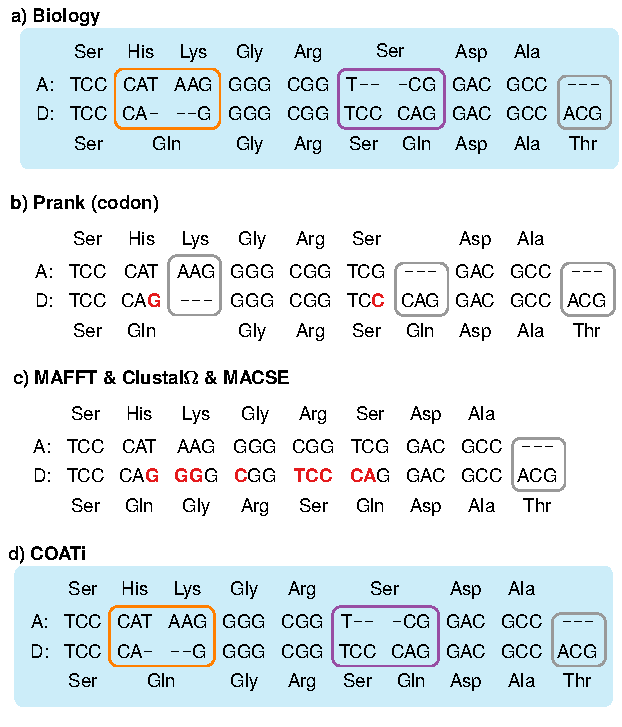
\includegraphics[scale=1]{fig-aln.pdf}
    \par
    \caption{
        Standard algorithms produce suboptimal alignments.
        (a) shows the true alignment of an ancestor sequence (A) and a descendant sequence (D).
        (b), (c), and (d) are the results of different aligners.
        Nucleotide mismatches are highlighted in red. Phase 0, phase 1, and phase 2 indels are shown in gray, purple, and orange, respectively.
        Additionally, the orange indel is type II (an amino-acid indel plus an amino-acid change) while the purple indel is type I (an amino-acid indel only).
        COATi is the only aligner able to retrieve the biological alignment in this example.
        }
    \label{fig:aln}
\end{figure}

Genome quality impacts conclusions drawn from comparative genomic studies, and uncorrected errors in the alignment stage can lead to erroneous results in comparative and functional genomic studies \citembethree{estimates_schneider_2009}{effect_fletcher_2010}{hubisz2011error}.
Genomes for model organisms often get refined over many iterations and achieve high quality with meticulously curated protein coding sequences.
In contrast, genomes for non-model organisms might only receive partial curation and typically have lower quality sequences and annotations.
These genomes often lack the amount of sequencing data needed to fix artifacts, including missing exons, erroneous mutations, and indels \citembe{jackman2018tigmint}.
%
When comparative and functional genomics studies include data from non-model organisms, care must be taken to identify and manage such artifacts; however,
current alignment methods are ill-equipped to handle common artifacts in genomic data, requiring costly curation practices that discard significant amounts of information.
To address this problem, we present COATi, short for COdon-aware Alignment Transducer, a pairwise statistical aligner that incorporates codon substitution models and is robust to artifacts present in modern genomic data.



\section*{Materials and Methods}

\DIFaddbegin \subsection*{\DIFadd{Statistical Alignment}}

\DIFaddend Statistical alignment is typically performed using pairwise hidden Markov models (pair-HMMs), which have the ability to rigorously model molecular sequence evolution \citembe{bradley2007transducers}.
Pair-HMMs are computational machines with two output tapes. Pair-HMMs contain a finite number of states---typically labeled match, insert, and delete---that emit symbols (nucleotides or amino acids) to one or both tapes.
Each tape represents a sequence, and a path through a pair-HMM is a possible pairwise alignment.
Conceptually, these machines generate two sequences ($\text{X}$ and $\text{Y}$) from an unknown ancestor and can calculate the probability that two sequences are related, represented by $P(\text{X}, \text{Y})$ \citembe{yoon_2009_hmm}.

A limitation of pair-HMMs is that they only model the evolution of two related sequences from an unknown ancestor.
Finite-state transducers (FSTs) have similar benefits to pair-HMMs with the additional feature that can model the generation of a descendant sequence given an ancestral one.
FSTs consume symbols from an input tape and emit symbols to an output tape.
Properly weighted, an FST can calculate the probability that a descendant sequence, $\text{Y}$, evolved from an ancestral sequence, $\text{X}$, represented by $P(\text{Y} | \text{X})$.
%DIF >  Furthermore, well-established algorithms for combining FSTs in different ways allow the design of complex models by combining simpler FSTs \citembe{bradley2007transducers}.
%DIF >  A powerful and versatile algorithm for comparative sequence analysis is composition, which consists of sending the output of one FST into the input of a second FST.
%DIF >  COATi uses composition to derive a statistical alignment model from the combination of smaller FSTs, each representing a specific process.
\DIFaddbegin 

\DIFaddend Furthermore, well-established algorithms for combining FSTs in different ways\DIFaddbegin \DIFadd{, including concatenation, composition, intersection, union, or reversal, }\DIFaddend allow the design of complex models by combining simpler FSTs \DIFdelbegin \DIFdel{\mbox{%DIFAUXCMD
\citembe{bradley2007transducers}}\hspace{0pt}%DIFAUXCMD
.
A }\DIFdelend \DIFaddbegin \DIFadd{\mbox{%DIFAUXCMD
\citep{bradley2007transducers,silvestre2021machine}}\hspace{0pt}%DIFAUXCMD
.
Specifically, composition is a }\DIFaddend powerful and versatile algorithm for comparative sequence analysis\DIFdelbegin \DIFdel{is composition, which consists }\DIFdelend \DIFaddbegin \DIFadd{, consisting }\DIFaddend of sending the output of one FST into the input of a second FST.
\DIFaddbegin \DIFadd{Composition allows combining two or more FSTs to create a new, more complex transducer. Figure \ref{fig:transcription} illustrates how DNA transcription for a codon can be achieved by composing a complementing FST with a transducer that replaces thymines with uracil, where the three nucleotides are read and complemented in \ref{fig:transcription}-a, which are then used as the input of \ref{fig:transcription}-b, resulting in the transcription of the codon (Fig.~\ref{fig:transcription}-c). }\DIFaddend COATi uses composition to derive a statistical alignment model from the combination of smaller FSTs, each representing a specific process.

\DIFaddbegin \begin{figure}[!ht]
    \centering
    \DIFaddFL{\hspace*{-3.5em}}\resizebox{1.05\textwidth}{!}{\definecolor{colorR}{RGB}{228,26,28}    % RED
\definecolor{colorB}{RGB}{55,126,184}   % BLUE
\definecolor{colorG}{RGB}{77,175,74}    % GREEN
\definecolor{colorP}{RGB}{152,78,163}   % PURPLE
\definecolor{colorO}{RGB}{255,127,0}    % ORANGE
\definecolor{colorY}{RGB}{255,255,51}   % YELLOW
\definecolor{colorBn}{RGB}{166,86,40}   % BROWN
\definecolor{colorPk}{RGB}{247,129,191} % PINK
\definecolor{colorGy}{RGB}{153,153,153} % GRAY

\tikzstyle{line}=[draw, -stealth', very thick]
\tikzstyle{block}=[circle,fill=colorB!50,on grid]
\tikzstyle{lab}=[]
\tikzstyle{w}=[lab,midway]
\tikzstyle{e}=[lab,midway,below=-4mm,auto=false,font=\scriptsize]

% \begin{document}
% \begin{tikzpicture}[node distance=25mm, auto]
\begin{tikzpicture}[node distance=25mm, auto,
	dottedline/.style = {ultra thick, loosely dotted,shorten >=1mm, shorten <=1mm}]

% complimenting FST
\node (titlea) {\textbf{a) DNA Complement}};

\node[block,below left=1cm and -10mm of titlea.west,fill=colorG!50] (start1) {start};
\node[block,right=15mm of start1,minimum size=20pt] (cod0) {};
\node[block,right=20mm of cod0,minimum size=20pt] (cod1) {};
\node[block,right=20mm of cod1,minimum size=20pt] (cod2) {};
\node[block,right=20mm of cod2,minimum size=20pt] (cod3) {};
\node[block,fill=colorR!50,right=15mm of cod3] (end1) {end};

\draw[line] (start1) -- (cod0);
\draw[line] (cod3) -- (end1);

\draw[line] (cod0) to[bend right=-60] node[e] {A:T} (cod1);
\draw[line] (cod0) to[bend right=-25] node[e] {C:G} (cod1);
\draw[line] (cod0) to[bend right=25] node[e,below=-4.5mm] {G:C} (cod1);
\draw[line] (cod0) to[bend right=60] node[e] {T:A} (cod1);

\draw[line] (cod1) to[bend right=-60] node[e] {A:T} (cod2);
\draw[line] (cod1) to[bend right=-25] node[e] {C:G} (cod2);
\draw[line] (cod1) to[bend right=25] node[e,below=-4.5mm] {G:C} (cod2);
\draw[line] (cod1) to[bend right=60] node[e] {T:A} (cod2);

\draw[line] (cod2) to[bend right=-60] node[e] {A:T} (cod3);
\draw[line] (cod2) to[bend right=-25] node[e] {C:G} (cod3);
\draw[line] (cod2) to[bend right=25] node[e,below=-4.5mm] {G:C} (cod3);
\draw[line] (cod2) to[bend right=60] node[e] {T:A} (cod3);

% T->U
\node[right=6cm of titlea] (titleb) {\textbf{b) Replacing thymine with uracil}};

\node[block,below right=1cm and 12mm of titleb.west,fill=colorG!50] (start2) {start};
\node[block,right=20mm of start2,minimum size=30pt] (cod4) {};
\node[block,fill=colorR!50,right=20mm of cod4] (end2) {end};

\draw[line] (start2) -- (cod4);
\draw[line] (cod4) -- (end2);

\draw[line] (cod4) to[out=165,in=105,min distance=2mm,looseness=5] node[e,below left=0.5mm and -6mm] {A:A} (cod4);
\draw[line] (cod4) to[out=85,in=15,min distance=2mm,looseness=5] node[e,below left=0.5mm and -1mm] {C:C} (cod4);
\draw[line] (cod4) to[out=-15,in=285,min distance=2mm,looseness=5] node[e,above left=0.5mm and -1mm] {G:G} (cod4);
\draw[line] (cod4) to[out=255,in=195,min distance=2mm,looseness=5] node[e,above left=0.5mm and -6mm] {T:U} (cod4);

% transcription FST
\node[below right=3cm and 25mm of titlea.west] (titlec) {\textbf{c) DNA Transcription}};

\node[block,below right=1cm and 1cm of titlec.west,fill=colorG!50] (start3) {start};
\node[block,right=15mm of start3,minimum size=20pt] (cod5) {};
\node[block,right=20mm of cod5,minimum size=20pt] (cod6) {};
\node[block,right=20mm of cod6,minimum size=20pt] (cod7) {};
\node[block,right=20mm of cod7,minimum size=20pt] (cod8) {};
\node[block,fill=colorR!50,right=15mm of cod8] (end3) {end};

\draw[line] (start3) -- (cod5);
\draw[line] (cod8) -- (end3);

\draw[line] (cod5) to[bend right=-60] node[e] {A:U} (cod6);
\draw[line] (cod5) to[bend right=-25] node[e] {C:G} (cod6);
\draw[line] (cod5) to[bend right=25] node[e,below=-4.5mm] {G:C} (cod6);
\draw[line] (cod5) to[bend right=60] node[e] {T:A} (cod6);

\draw[line] (cod6) to[bend right=-60] node[e] {A:U} (cod7);
\draw[line] (cod6) to[bend right=-25] node[e] {C:G} (cod7);
\draw[line] (cod6) to[bend right=25] node[e,below=-4.5mm] {G:C} (cod7);
\draw[line] (cod6) to[bend right=60] node[e] {T:A} (cod7);

\draw[line] (cod7) to[bend right=-60] node[e] {A:U} (cod8);
\draw[line] (cod7) to[bend right=-25] node[e] {C:G} (cod8);
\draw[line] (cod7) to[bend right=25] node[e,below=-4.5mm] {G:C} (cod8);
\draw[line] (cod7) to[bend right=60] node[e] {T:A} (cod8);

\end{tikzpicture}}
    \caption[DNA Transcription via FST Composition]{\DIFaddFL{DNA transcription via FST composition. The composition of (a) a codon complimenting FST and (b) an FST that replaces T with U generates (c) an FST that implements codon transcription ($a~\circ$~b = c).}}
    \label{fig:transcription}
\end{figure}

\DIFaddend COATi implements the pairwise alignment of a potentially lower-quality sequence against a high-quality sequence as a path through the Evolution FST (Fig.\ \ref{fig:evolution-fst}) \citep[c.f.][]{holmes2001evolutionary}.
Here, COATi treats the high-quality (reference) sequence as the ``ancestor'' and the potentially lower-quality sequence as the ``descendant''.
\DIFdelbegin \DIFdel{This }\DIFdelend \DIFaddbegin \DIFadd{The assumption is that the reference sequence is in-phase, which is used to help preserve the reading frame and safeguard against possible frameshifts in the ``descendant''. Therefore, the high-quality sequence must not contain incomplete codons (the number of nucleotides is multiple of three) and be free of any ambiguous nucleotides or early stop codons. In contrast, the potentially lower-quality sequence has no such restrictions and can be of any length, contain early stop codons---treated as artifacts---, and include ambiguous codons.
}

\DIFadd{The Evolution }\DIFaddend FST is the result of composing a substitution FST that encodes a codon model (Fig.\ \ref{fig:evolution-fst}-a) and an indel FST that models insertions and deletions, including frameshifts (Fig.\ \ref{fig:evolution-fst}-b).
A key innovation of this FST, with respect to others, is the combination of a codon substitution model with a nucleotide-based geometric indel model that allows gaps to occur at any position.

\DIFaddbegin \begin{figure}[h!]
\centering
\setlength{\columnsep}{-3cm}
\begin{multicols}{2}
    \DIFaddFL{\hspace*{-2.8cm}}\resizebox{0.55\textwidth}{!}{\definecolor{colorR}{RGB}{228,26,28}    % RED
\definecolor{colorB}{RGB}{55,126,184}   % BLUE
\definecolor{colorG}{RGB}{77,175,74}    % GREEN
\definecolor{colorP}{RGB}{152,78,163}   % PURPLE
\definecolor{colorO}{RGB}{255,127,0}    % ORANGE
\definecolor{colorY}{RGB}{255,255,51}   % YELLOW
\definecolor{colorBn}{RGB}{166,86,40}   % BROWN
\definecolor{colorPk}{RGB}{247,129,191} % PINK
\definecolor{colorGy}{RGB}{153,153,153} % GRAY

\tikzstyle{line}=[draw, -stealth', very thick]
\tikzstyle{block}=[circle,fill=colorB!50,on grid]
\tikzstyle{lab}=[]
\tikzstyle{w}=[lab,midway]
\tikzstyle{e}=[lab,midway,above=0.2mm,auto=false,font=\scriptsize]

% \begin{document}
% \begin{tikzpicture}[node distance=25mm, auto]
\begin{tikzpicture}[node distance=25mm, auto,
	dottedline/.style = {ultra thick, loosely dotted,shorten >=1mm, shorten <=1mm}]
%%% MG94 marginal substitution FST
% \node (titlea) {};

\node[block,fill=colorG!50] (start_sub) {start};
\node[block,right=15mm of start_sub] (S_sub) {M};
\node[block,right=75mm of S_sub] (M_sub) {S};
\node[block,fill=colorR!50,right=15mm of M_sub] (end_sub) {end};

% AAA->AAA
\node[block,above right=12mm and 20mm of S_sub,minimum size=15pt] (s2) {};
\node[block,above right=3mm and 20mm of s2,minimum size=15pt] (s1) {};
% % AAA->AAC
\node[block,above right=4mm and 20mm of S_sub,minimum size=15pt] (s4) {};
\node[block,below right=-1mm and 20mm of s4,minimum size=15pt] (s3) {};
% TTT->TTT
\node[block,below right=6mm and 20mm of S_sub,minimum size=15pt] (s122) {};
\node[block,below right=3mm and 20mm of s122,minimum size=15pt] (s121) {};

\draw[line] (start_sub) -- (S_sub);
\draw[line] (S_sub) to[bend right=40] (M_sub);
\draw[line] (M_sub) -- (end_sub);

% AAA->AAA
% \draw[line] (M_sub) to[bend right=15] node[w,pos=0.7,above right=3mm and 1mm,font=\scriptsize,rotate=-20] {$P(AAA|AAA)$} (s1);
\draw[line] (M_sub) to[bend right=15] node[e,pos=0.4,rotate=-20] {A:A/$P(AAA|AAA)$} (s1);
\draw[line] (s1) to[bend right=15] node[e,pos=0.5] {A:A} (s2);
\draw[line] (s2) to[bend right=15] node[e,pos=0.5] {A:A} (S_sub);

% % AAA->AAC
\draw[line] (M_sub) to[bend right=5] node[e,pos=0.5,rotate=-8,below=-5mm] {A:A/$P(AAC|AAA)$} (s3);
\draw[line] (s3) to[bend right=8] node[e,pos=0.5] {A:A} (s4);
\draw[line] (s4) to[bend right=8] node[e,pos=0.5] {A:C} (S_sub);

\node[below=9mm of s1,font=\Huge] {$\vdots$};
\node[below=5mm of s2,font=\Huge] {$\vdots$};

% TTT->TTT
% \draw[line] (M_sub) to[bend right=-5] node[w,pos=0.5,above right=1mm and -11mm, rotate=5,font=\scriptsize] {$P(TTT|TTT)$} (s121);
\draw[line] (M_sub) to[bend right=-5] node[e,pos=0.5,rotate=9] {T:T/$P(TTT|TTT)$} (s121);
\draw[line] (s121) to[bend right=-5] node[e,pos=0.5] {T:T} (s122);
\draw[line] (s122) to[bend right=-5] node[e,pos=0.4] {T:T} (S_sub);
\end{tikzpicture}}
    \columnbreak
    \resizebox{0.55\textwidth}{!}{\definecolor{colorR}{RGB}{228,26,28}    % RED
\definecolor{colorB}{RGB}{55,126,184}   % BLUE
\definecolor{colorG}{RGB}{77,175,74}    % GREEN
\definecolor{colorP}{RGB}{152,78,163}   % PURPLE
\definecolor{colorO}{RGB}{255,127,0}    % ORANGE
\definecolor{colorY}{RGB}{255,255,51}   % YELLOW
\definecolor{colorBn}{RGB}{166,86,40}   % BROWN
\definecolor{colorPk}{RGB}{247,129,191} % PINK
\definecolor{colorGy}{RGB}{153,153,153} % GRAY

\tikzstyle{line}=[draw, -stealth', very thick]
\tikzstyle{block}=[circle,fill=colorB!50,on grid]
\tikzstyle{lab}=[]
\tikzstyle{w}=[lab,midway]
\tikzstyle{e}=[lab,midway,above=0.2mm,auto=false,font=\small]

\begin{tikzpicture}[node distance=40mm, auto,
	dottedline/.style = {ultra thick, loosely dotted,shorten >=1mm, shorten <=1mm}]

%%% Indel FST
% \node[below left=3cm and -14mm of titlea.east] (titleb) {\textbf{b) Insertion-Deletion}};
\node (titleb) {};

\node[block,below right=1.5cm and -1.5cm of titleb.center,fill=colorG!50] (start1) {start};
\node[block,below=15mm of start1] (S1) {M};
\node[block,below=of S1] (I1) {U};
\node[block,right=of I1] (U1) {I};
\node[block,above=of U1] (W1) {W};
\node[block,above=20mm of W1] (D1) {V};
\node[block,right=of D1] (V1) {D};
\node[block,right=of W1] (M1) {S};
\node[block,fill=colorR!50,right=20mm of M1] (end1) {end};

\draw (D1) +(0mm,-20mm) coordinate (C1);
\draw (D1) +(50mm,-10mm) coordinate (C2);
\draw[line] (start1) -- (S1);
\draw[line] (S1) -- node[w] {$g$} (I1);
\draw[line] (S1) -- node[w] {$1-g$} (W1);
\draw[line] (U1) to[out=120,in=60]  node[w,above] {$e$} (I1);
\draw[line] (U1) -- node[w,pos=0.1,right] {$1-e$} (W1);
\draw[line] (W1) -- node[w] {$g$} (D1);
\draw[line] (W1) -- node[w] {$1-g$} (M1);
\draw[line] (M1) -- node[w] {} (end1);
\draw[line] (V1) to[out=120,in=60] node[w,above] {$e$} (D1);
\draw[line] (V1) -- node[w] {$1-e$} (M1);
%insertions
\draw[line] (I1) to[bend right=-25] node[e,pos=0.48,below=-5mm] {\O:A/$\grande{\pi}_{\text{A}}$} (U1);
\draw[line] (I1) to[bend right=0] node[e,pos=0.48,below=-5mm] {\O:C/ $\grande{\pi}_{\text{C}}$} (U1);
\draw[line] (I1) to[bend right=25] node[e,pos=0.48,below=-5mm] {\O:G/ $\grande{\pi}_{\text{G}}$} (U1);
\draw[line] (I1) to[bend right=50] node[e,pos=0.48,below=-5mm] {\O:T/ $\grande{\pi}_{\text{T}}$} (U1);
% deletion
\draw[line] (D1) to[bend right=-25] node[e,pos=0.5,below=-4.5mm] {A:\O} (V1);
\draw[line] (D1) to[bend right=0] node[e,pos=0.5,below=-4.5mm] {C:\O} (V1);
\draw[line] (D1) to[bend right=25] node[e,pos=0.5,below=-4.5mm] {G:\O} (V1);
\draw[line] (D1) to[bend right=50] node[e,pos=0.5,below=-4.5mm] {T:\O} (V1);
% A -> {A,C,G,T}
\draw[line] (M1) to[bend left=25] (S1);
\draw[line] (M1) to[bend left=35] (S1);
\draw[line] (M1) to[bend left=45] (S1);
\draw[line] (M1) to[bend left=55] (S1);
\path[] (M1) to[bend left=25] node[e,pos=0.8,below=-3mm,fill=white] {A:A} (S1);
\path[] (M1) to[bend left=35] node[e,pos=0.6,below=-3mm,fill=white] {C:C} (S1);
\path[] (M1) to[bend left=45] node[e,pos=0.4,below=-3mm,fill=white] {G:G} (S1);
\path[] (M1) to[bend left=55] node[e,pos=0.2,below=-3mm,fill=white] {T:T} (S1);
% % dots
% \node[below left=9mm and -1mm of W1,font=\Huge] {$\vdots$};
% % T -> {A,C,G,T}
% \draw[line] (M1) to[bend left=55] (S1);
% \draw[line] (M1) to[bend left=59] (S1);
% \draw[line] (M1) to[bend left=63] (S1);
% \draw[line] (M1) to[bend left=67] (S1);
% \path[] (M1) to[bend left=55] node[e,pos=0.8,below=-3mm,fill=white] {T:A} (S1);
% \path[] (M1) to[bend left=59] node[e,pos=0.6,below=-3mm,fill=white] {T:C} (S1);
% \path[] (M1) to[bend left=63] node[e,pos=0.4,below=-3mm,fill=white] {T:G} (S1);
% \path[] (M1) to[bend left=67] node[e,pos=0.2,below=-3mm,fill=white] {T:T} (S1);

%%%% Base calling error FST
% \node[right=6cm of titleb.east] (titlec) {\textbf{Base Calling Error}};

% \node[block,below=1.5cm of titlec,fill=colorG!50] (start_bce) {start};
% \node[block,right=15mm of start_bce] (S_bce) {M};
% \node[block,right=60mm of S_bce] (M_bce) {S};
% \node[block,fill=colorR!50,right=15mm of M_bce] (end_bce) {end};

% \draw[line] (start_bce) -- (S_bce);
% \draw[line] (M_bce) -- (end_bce);

% % \draw[line] (M_bce) to[bend right=25] node[w,below=1mm,pos=0.66] {$\varepsilon$} (S_bce);
% \draw[line] (M_bce) to[bend right=25] node[e] {y$_\text{i}$:z$_\text{j}$/$\grande{\varepsilon}$} (S_bce);
% % \draw[line] (M_bce) to node[w,below=0.2mm,pos=0.66] {$1 - 3 \cdot \varepsilon$} (S_bce);
% \draw[line] (M_bce) to node[e] {y$_\text{i}$:z$_\text{j}$/$1-3\cdot \grande{\varepsilon}$} (S_bce);
% \draw[line] (M_bce) to[bend right=-25] (S_bce);
% \draw[line] (M_bce) to[bend right=-25] node[e] {y$_\text{i}$:N} (S_bce);

% \draw[line] (S_bce) to[bend left=-60] (M_bce);

%%% Legend

% \node[below left=2cm and 1.5cm of start_bce,text width=50mm,anchor=north west] (sequences) {
\node[below right=5.8cm and 4.5cm of titleb,text width=50mm,anchor=north west] (sequences) {
\begin{tabular}{r@{\,: }l}
\multicolumn{2}{l}{\textbf{Parameters}}\\
    \hline
	% X & input nucleotides\\
	% y & input sequence\\
	% z & output sequence\\
	\O & empty sequence\\
	$g$ & gap open weight\\
	$e$ & gap extension weight\\
	$\grande{\pi}$ & residue stationary freq.\\
        % Y$_i$:Y$_i$ & matches\\
        % Y$_i$:Y$_j$ & mismatches\\
 % 	$i \rightarrow i$ & matching input to intermediate base\\
	% $i \rightarrow j$ & mismatching input to intermediate base\\
	% $i \rightarrow N$ & input to intermediate ambiguous base N\\
\end{tabular}
};

\end{tikzpicture}}
\end{multicols}
\par
\caption{\DIFaddFL{The Evolution FST is assembled by composing a substitution FST and an indel FST.
Each node represents a state in an FST while arcs display possible transitions between states (and their weights). Unlabeled arcs have weights of 1.
(a) The substitution FST encodes a $61 \times 61 $ codon substitution model with 3721 arcs from S to M. These arcs consume three nucleotides from the input tape and emit three nucleotides to the output tape. The weight of each arc is a conditional probability derived from a codon substitution model.
(b) The indel FST allows for insertions (U to I) and deletions (V to D). Insertion arcs are weighted according to the codon model's stationary distribution of nucleotides, and deletion arcs have a weight of 1. On top of the indel FST, we add a base-calling-error FST (Supplemental Materials Figure 1) to model sequencing errors. Contiguous insertions and deletions are always arranged for insertions to precede deletions to limit equivalent alignments.}}
\label{fig:evolution-fst}
\end{figure}

\DIFaddend Composing both sequences with the Evolution FST results in the transducer of all possible alignments.
Any path through this FST represents a pairwise alignment, while the shortest path (by weight) corresponds to the best alignment.
\DIFaddbegin \DIFadd{When equally optimal alignments exist, ties are broken according to the FST shortest-path algorithm.
An example of an FST-based alignment can be found in Supplementary Materials Figure 2.
}\DIFaddend All FST operations in COATi, including model development, composition, search for the shortest path, and other optimization algorithms, are performed using the C++ openFST library \citembe{allauzen2007openfst}.
However, the Evolution FST has a large state space to keep track of codon substitution rates when codons might be interspersed with indel events. This additional state space increases the computational complexity of the alignment algorithm.

\DIFdelbegin %DIFDELCMD < \begin{figure}[h!]
%DIFDELCMD < \centering
%DIFDELCMD < 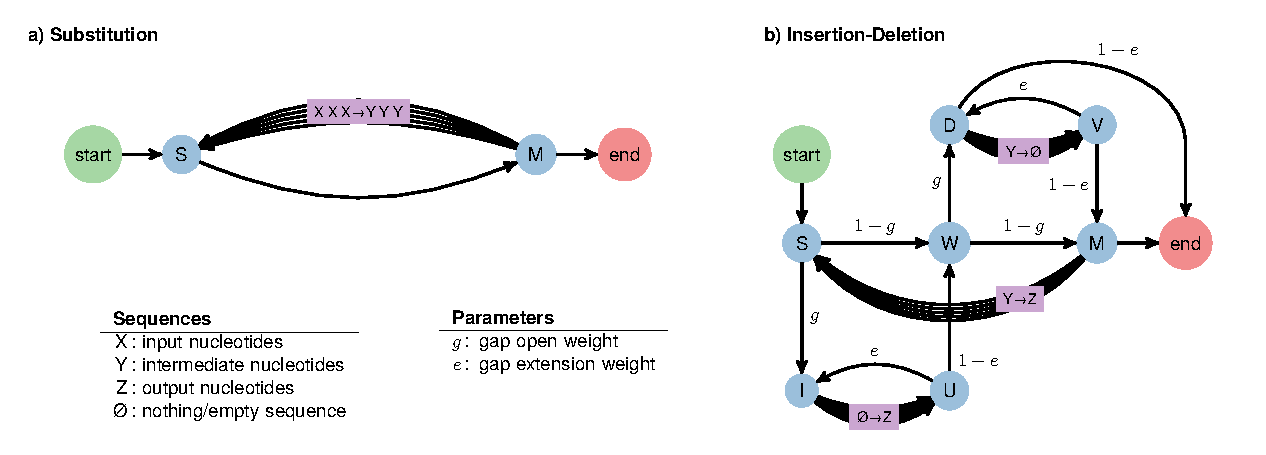
\includegraphics[width=\textwidth]{fig-evolution-fst.pdf}
%DIFDELCMD < \par
%DIFDELCMD < %%%
%DIFDELCMD < \caption{%
{%DIFAUXCMD
\DIFdelFL{The Evolution FST is assembled by composing a substitution FST and an indel FST.
Each node represents a state in an FST while arcs display possible transitions between states (and their weights). Unlabeled arcs have weights of 1.
(a) The substitution FST encodes a $61 \times 61 $ codon substitution model with 3721 arcs from M to S. These arcs consume three nucleotides from the input tape and emit three nucleotides to the output tape. The weight of each arc is a conditional probability derived from a codon substitution model.
(b) The indel FST allows for insertions (I to U) and deletions (D to V). Insertion arcs are weighted according to the codon model's stationary distribution of nucleotides, and deletion arcs have a weight of 1. On top of the indel FST, we add a base-calling-error FST (Supplemental Materials Figure 5) to model sequencing errors. Contiguous insertions and deletions are always arranged for insertions to precede deletions to limit equivalent alignments.}}
%DIFAUXCMD
%DIFDELCMD < \label{fig:evolution-fst}
%DIFDELCMD < \end{figure}
%DIFDELCMD < %%%
\DIFdelend \DIFaddbegin \section*{\DIFadd{Codon Substitution Models}}
\DIFaddend 

Codon substitution models are uncommon in sequence aligners, despite their extensive use in phylogenetics.
COATi implements the Muse and Gaut (\citeyear{muse_gaut_1994}) codon model (codon-triplet-mg) and the Empirical Codon Model \citembe{kosiol_ECM_2007} (codon-triplet-ecm).
It also lets the user provide a codon substitution matrix.
The default FST model (codon-triplet-mg) does not allow early stop codons in the ancestor sequence; although, it does support mutations to (early) stop codons under the assumption that these are artifacts common in low-quality data.

To reduce the runtime complexity of COATi, we have also developed an approximation of the Evolution FST that can be implemented with standard dynamic programming techniques. This approximation uses a marginal substitution model where the output nucleotides are independent of one another and only depend on the input codon and position. This produces a $\left(61 \times 3 \right) \times 4$ substitution model and eliminates the need to track dependencies between output nucleotides.

A marginal substitution model is calculated from a standard substitution model by calculating the marginal probabilities that each ancestral codon produces specific descendant nucleotides at each reading frame position.
%
Specifically, let
$P_\text{cod}\left(Y_0 \cdot Y_1 \cdot Y_2 \middle| X_0 \cdot X_1 \cdot X_2\right)$ represent transition probabilities from a standard codon model, and
%
\[
P_\text{mar}\left(Y_p = y \middle| X_0 \cdot X_1 \cdot X_2\right) =
\sum_{Y_0 \cdot Y_1 \cdot Y_2} I(Y_p = y) P_\text{cod}\left(Y_0 \cdot Y_1 \cdot Y_2 \middle| X_0 \cdot X_1 \cdot X_2\right)
\]
%
represent the marginal transition probabilities, where
$p \in \{0, 1, 2\}$ is the position of the descendant nucleotide relative to the ancestral reading frame and $I$ is an indicator function defined
%
$I(e) = \{ 1 \text{ if $e$ is true and } 0 \text{ otherwise}\}$.
%
COATi contains marginal models for both Muse and Gaut (\citeyear{muse_gaut_1994}) or the Empirical Codon Model, resulting in the marginal models codon-marginal-mg (default model) and codon-marginal-ecm.
These models emphasize the position in a codon where the substitution occurs, help restrict the effects of low-quality data in the descendant sequence, and allow more than one substitution per codon.
In combination with the indel model, alignment using the marginal model is implemented using dynamic programming.

\DIFdelbegin \section*{\DIFdel{Results and Discussion}}
%DIFAUXCMD
\DIFdel{Using }\DIFdelend \DIFaddbegin \subsection*{\DIFadd{Empirical Simulation Algorithm}}

\DIFadd{I downloaded }\DIFaddend 16000 human genes and their gorilla orthologs from the ENSEMBL
database \DIFdelbegin \DIFdel{\mbox{%DIFAUXCMD
\citembe{ensembl_hubbard_2002}}\hspace{0pt}%DIFAUXCMD
, we simulated a data set of pairwise
alignments with empirical gap patterns.
We used the data set to evaluate the accuracy of COATi and a suite of popular aligners spanning multiple alignment methods:
Clustal$\Omega$ v1.2.4 \mbox{%DIFAUXCMD
\citembe{clustal_omega_sievers_2011}}\hspace{0pt}%DIFAUXCMD
,
MACSE v2.06 \mbox{%DIFAUXCMD
\citembe{ranwez_macse_2011}}\hspace{0pt}%DIFAUXCMD
, MAFFT v7.505
\mbox{%DIFAUXCMD
\citembe{katoh2013mafft}}\hspace{0pt}%DIFAUXCMD
, and PRANK v.150803 \mbox{%DIFAUXCMD
\citembe{prank_loytynoja_2014}}\hspace{0pt}%DIFAUXCMD
.
}%DIFDELCMD < 

%DIFDELCMD < %%%
\DIFdelend \DIFaddbegin \DIFadd{\mbox{%DIFAUXCMD
\citep{ensembl_hubbard_2002}}\hspace{0pt}%DIFAUXCMD
.
}\DIFaddend After downloading, \DIFdelbegin \DIFdel{we }\DIFdelend \DIFaddbegin \DIFadd{I }\DIFaddend removed 2232 sequence-pairs longer than 6000 nucleotides and \DIFdelbegin \DIFdel{then }\DIFdelend aligned the remaining pairs with all five methods.
At least one aligner added gaps to \DIFdelbegin \DIFdel{6007 }\DIFdelend \DIFaddbegin \DIFadd{6048 }\DIFaddend sequence pairs, and no aligner added gaps to 7761 sequence pairs.
\DIFdelbegin \DIFdel{We then }\DIFdelend \DIFaddbegin \DIFadd{Then, I }\DIFaddend randomly introduced gap patterns extracted from all five methods into the ungapped sequence pairs to generate the benchmark alignments.
\DIFdelbegin \DIFdel{The accuracy of inferred alignments compared to the benchmarks was measured using \mbox{%DIFAUXCMD
\citeauthor{metrics_blackburne_whelan_2011}}\hspace{0pt}%DIFAUXCMD
's \mbox{%DIFAUXCMD
\citeyearpar{metrics_blackburne_whelan_2011} }\hspace{0pt}%DIFAUXCMD
distance metric, $d_{seq}$.
Additionally, because different alignments may be evolutionary equivalent }\DIFdelend \DIFaddbegin 

\DIFadd{The simulation algorithm can introduce a pairwise alignment pattern to any two nucleotide sequences of equal length. The alignment pattern is given as a CIGAR string (Compact Idiosyncratic Gapped Alignment Report), a format commonly used to summarize aligned reads to a reference genome. Assigning one of the sequences as the reference, to distinguish between insertions and deletions, CIGAR strings can also summarize pairwise alignments by grouping the number of contiguous matches or mismatches `M'}\DIFaddend , \DIFdelbegin \DIFdel{we scored }\DIFdelend \DIFaddbegin \DIFadd{deletions `D', and insertions `I'. The resulting pattern combines these letters preceded by the number of characters for each section as they appear in the alignment. This pattern is introduced by replacing nucleotides with gaps as indicated by deletions on one sequence and randomly introducing residues where the CIGAR strings indicated insertions.
}

%DIF >  Several safety checks are in place to ensure the algorithm runs correctly and the result is accurate. The assertions are divided into checking lengths and maintaining the reading frame of each section. The simulation can fail if the length of the sequences is different or if, without counting insertions, the length of the pattern to be inserted is longer. In addition, maintaining the phases of each section in the CIGAR string is important to avoid introducing errors such as frameshifts. 

\DIFadd{I created the benchmark of alignments by using an equal number of randomly sampled gap patterns from each aligner.
%DIF >  After creating the dataset, I removed the gaps and measured how well different aligners were able to retrieve the true alignments.
I used the dataset to evaluate the accuracy of COATi and a suite of popular aligners spanning various alignment methods:
Clustal$\Omega$ v1.2.4 \mbox{%DIFAUXCMD
\citep{clustal_omega_sievers_2011}}\hspace{0pt}%DIFAUXCMD
,
MACSE v2.06 \mbox{%DIFAUXCMD
\citep{ranwez_macse_2011}}\hspace{0pt}%DIFAUXCMD
, MAFFT v7.505
\mbox{%DIFAUXCMD
\citep{katoh2013mafft}}\hspace{0pt}%DIFAUXCMD
, and PRANK v.150803 \mbox{%DIFAUXCMD
\citep{prank_loytynoja_2014}}\hspace{0pt}%DIFAUXCMD
.
}

\subsection*{\DIFadd{Metrics}}

\DIFadd{To quantify the similarity between each alignment in the benchmark and the corresponding output obtained by the different tools, I used the alignment error metric $d_{seq}$ \mbox{%DIFAUXCMD
\citep{metrics_blackburne_whelan_2011}}\hspace{0pt}%DIFAUXCMD
. This metric accounts for indels and is more informative than conventional distance scores like sum-of-pairs or total columns. Intuitively, $d_{seq}$ ranges between zero and one and can be interpreted as the probability that a randomly selected residue will be aligned to a different location against a sequence that does not contain such residue.
}

\DIFadd{The computation of $d_{seq}$ involves characterizing the gaps present in the alignment. Then, a site-wise homology set $H(A)^i_j$ is calculated for each alignment $A$, sequence $i$, and character $j$. The distance between two alignments $A$ and $B$ is the average across all characters of the symmetric difference (or Hamming distance), represented as `$\triangle$' between homology sets over the length of such sets:
}

\begin{equation}
\DIFadd{d(A,B) = \frac{1}{c} \sum_i \sum_j \frac{|H(A)^i_j \triangle H(B)^i_j|}{|H(A)^i_j|+|H(B)^i_j|}
}\end{equation}

\noindent \DIFadd{where $c$ is the sum of the sequence lengths.
}

\DIFadd{In addition, I compared the number of perfectly and imperfectly retrieved alignments for each aligner. Perfect alignments are defined as those with a distance of zero to the reference alignment ($d_{seq} = 0$), indicating 100\% similarity. Notably, a set of sequences can have more than one optimal alignment under the same evolutionary model (same score), despite algorithms typically producing a single result. Consequently, to account for evolutionary equivalent alignments, I scored all }\DIFaddend alignments using the \DIFdelbegin \DIFdel{codon-marginal-mg model , and any alignment that had the same score as the benchmark alignment was considered equivalent to the benchmark alignment .
The accuracy of identifying }\DIFdelend \DIFaddbegin \DIFadd{marginal model and also considered perfect those with scores identical to the benchmark.
Furthermore, I counted the number of alignments with the lowest distance $d_{seq}$ to the true alignment, including ties, reported as best alignments. Moreover, I computed the count of imperfect alignments, where an alignment is considered imperfect when its distance to the reference alignment is greater than zero ($d_{seq} > 0$) and another method successfully produced an alignment with 100\% similarity. This analysis exposes instances where all aligners fall short of achieving a perfect result in addition to a direct comparison.
}

%DIF >  \cyan{The first sentence intro is a good idea, but rewrite!}
%DIF >  Sequencing artifacts and errors made in alignment can lead to inaccurate results in genomics. This is especially true in studies of positive selection and positively selected genes.

\DIFadd{To evaluate how well the aligners were able to identify }\DIFaddend positive and negative selection\DIFdelbegin \DIFdel{was calculated using the $F_1$ score by estimating }\DIFdelend \DIFaddbegin \DIFadd{, I estimated }\DIFaddend $k_s$ and $k_a$ statistics\DIFdelbegin \DIFdel{\mbox{%DIFAUXCMD
\citembe{ka_ks_li_1993} }\hspace{0pt}%DIFAUXCMD
(Supplementary Methods) }\DIFdelend . \DIFdelbegin \DIFdel{The $F_1$ score evaluates the accuracy of a model by assigning equal importance to precision }\DIFdelend \DIFaddbegin \DIFadd{$k_s$ }\DIFaddend and \DIFdelbegin \DIFdel{recall, and }\DIFdelend \DIFaddbegin \DIFadd{$k_a$ are, respectively, the number of substitutions per synonymous site (no changes at the amino acid level) and per non-synonymous site (introduces changes at the amino acid level) between two protein-coding genes. They are also denoted as $d_s$ and $d_n$ in the literature. I used the R package seqinr \mbox{%DIFAUXCMD
\citep{seqinr} }\hspace{0pt}%DIFAUXCMD
to estimate these metrics, which follows the popular method put forth by Li \mbox{%DIFAUXCMD
\citep{ka_ks_li_1993}}\hspace{0pt}%DIFAUXCMD
. First, this method takes two aligned homologous protein-coding sequences and classifies the nucleotide sites in a sequence as nondegenerate, twofold degenerate, and fourfold degenerate. A site is nondegenerate if all possible changes at that site are nonsynonymous, twofold degenerate if one of the three possible changes is synonymous, and fourfold degenerate if all possible changes are synonymous. Second, the nucleotide changes between the two sequences are counted and divided as transitional (A$\leftrightarrow$G, C$\leftrightarrow$T) and transversional (\{A, G\}$\leftrightarrow$\{C, T\}). Third, the Kimura two-parameter distance \mbox{%DIFAUXCMD
\citep{kimura1980simple} }\hspace{0pt}%DIFAUXCMD
is used to estimate the number of transitions and transversions per site type (nondegenerate, twofold degenerate, and fourfold degenerate), which is used as a correction factor for multiple hits. Finally, $k_s$ is the estimate of the average transitional rate at twofold and fourfold degenerate sites, and $k_a$ is the estimate of the average transversional rate at nondegenerate and twofold sites. In the results, these metrics are reported as the F$_1$ score, which is the harmonic mean of precision (true positives over total positives) and recall (true positives over true positives and false negatives). This score }\DIFaddend ranges between 0 and 1, with a score of 1 representing a perfect result.

\DIFaddbegin \DIFadd{In addition, we compared the estimated evolutionary distance between the reference and inferred alignments using the Kimura 2-parameter model \mbox{%DIFAUXCMD
\citep{kimura1980simple}}\hspace{0pt}%DIFAUXCMD
. The calculation of the Kimura 2-parameter model involves considering the rates of nucleotide transitions and transversions. The formula used for distance calculation is $D = -0.5 \cdot \log((1 - 2P - Q) \cdot \sqrt{1 - 2Q})$, where $P$ represents the proportion of transitional substitutions and $Q$ represents the proportion of transversional substitutions. The resulting distance provides a quantitative measure of the evolutionary divergence between the sequences. These calculations were performed using the R software package ape \mbox{%DIFAUXCMD
\citep{paradis2019ape}}\hspace{0pt}%DIFAUXCMD
.
}

\section*{\DIFadd{Results and Discussion}}
%DIF >  Using 16000 human genes and their gorilla orthologs from the ENSEMBL
%DIF >  database \citembe{ensembl_hubbard_2002}, we simulated a data set of pairwise
%DIF >  alignments with empirical gap patterns.
%DIF >  We used the data set to evaluate the accuracy of COATi and a suite of popular aligners spanning multiple alignment methods:
%DIF >  Clustal$\Omega$ v1.2.4 \citembe{clustal_omega_sievers_2011},
%DIF >  MACSE v2.06 \citembe{ranwez_macse_2011}, MAFFT v7.505
%DIF >  \citembe{katoh2013mafft}, and PRANK v.150803 \citembe{prank_loytynoja_2014}.

%DIF >  After downloading, we removed 2232 sequence-pairs longer than 6000 nucleotides and then aligned the remaining pairs with all five methods.
%DIF >  At least one aligner added gaps to 6048 sequence pairs, and no aligner added gaps to 7719 sequence pairs.
%DIF >  We then randomly introduced gap patterns extracted from all five methods into the ungapped sequence pairs to generate the benchmark alignments.
%DIF >  The accuracy of inferred alignments compared to the benchmarks was measured using \citeauthor{metrics_blackburne_whelan_2011}'s \citeyearpar{metrics_blackburne_whelan_2011} distance metric, $d_{seq}$.
%DIF >  Additionally, because different alignments may be evolutionary equivalent, we scored alignments using the codon-marginal-mg model, and any alignment that had the same score as the benchmark alignment was considered equivalent to the benchmark alignment.
%DIF >  The accuracy of identifying positive and negative selection was calculated using the $F_1$ score by estimating $k_s$ and $k_a$ statistics
%DIF >  \citembe{ka_ks_li_1993} (Supplementary Methods).
%DIF >  The $F_1$ score evaluates the accuracy of a model by assigning equal importance to precision and recall, and ranges between 0 and 1, with a score of 1 representing a perfect result.

\DIFadd{COATi, using the codon-triplet-mg model, obtained better results compared to a wide variety of alignment strategies.
It was significantly more accurate (lower $d_{seq}$) at inferring the empirically simulated alignments compared to other methods; all p-values were less than $1.3 \cdot 10^{-76}$ according to the one-tailed, paired Wilcoxon signed-rank tests (Supplementary Materials Figure 1).
%DIF > 
In addition, COATi produced more perfect alignments, less imperfect alignments, and more accurately inferred events of positive and negative selection (Table \ref{table:comp}). Furthermore, the estimated evolutionary divergence from the alignments retrieved by COATi is substantially less overestimated than other methods (Table \ref{table:comp}, Supplemental Materials Figure 8).
}

\DIFadd{Clustal$\Omega$ generated alignments via amino acid translations and obtained the highest average alignment error while having difficulties retrieving positive selection.
MACSE used a DNA-AA hybrid model, allowing frameshifts, and obtained similar results to MAFFT using a DNA model.
PRANK, using a codon model, had an average alignment error between MACSE/MAFFT and Clustal$\Omega$ but was unable to generate alignments for some sequence pairs.
}

\DIFaddend % Software comparison table
\begin{table}[!ht]
\centering
% \begin{table}[h!]
% \begin{adjustbox}{width=\columnwidth,center}
\definecolor{bestcolor}{RGB}{230,230,230}

\begingroup\centering
\begin{tabular}{r|ccccc}
      & \textbf{COATi} & \textbf{MAFFT} & \textbf{PRANK\textsuperscript{*}} & \textbf{MACSE} & \textbf{Clustal$\Omega$}\\
\hline
Method    & Trip-MG & DNA & Codon & DNA+AA & AA\\[2pt]
%\hline
Avg alignment error ($d_{seq}$) & \cellcolor{bestcolor}0.00221 & 0.01471 & 0.01828 & 0.01399 & 0.02929\\
Best alignments & \cellcolor{bestcolor}5139 & 4692 & 4774 & 3737 & 2615\\
Perfect alignments & \cellcolor{bestcolor}5793 & 5292 & 4725 & 2861 & 2893\\
Imperfect alignments & \cellcolor{bestcolor}1048 & 1549 & 2116 & 3980 & 3948\\
% \hline
F1 score for positive selection & \cellcolor{bestcolor}98.1\pct & 84.3\pct & 86.7\pct & 79.5\pct & 68.7\pct\\
F1 score for negative selection & \cellcolor{bestcolor}99.8\pct & 98.4\pct & 98.7\pct & 98.2\pct & 96.9\pct\DIFaddbeginFL \\
\DIFaddFL{Overestimated K2P distances }& \cellcolor{bestcolor}{10.9}\pct & \DIFaddFL{26.6}\pct & \DIFaddFL{33.8}\pct & \DIFaddFL{48.7}\pct & \DIFaddFL{61.8}\pct
\DIFaddendFL \end{tabular}
\par\endgroup
% \end{adjustbox}
% \end{table}

%DIF >  "Model COATi overestimated 10.9% of branch lengths; mean 0.0075 +/- 0.0052"
%DIF >  "Model MAFFT overestimated 26.6% of branch lengths; mean 0.017 +/- 0.0339"
%DIF >  "Model PRANK overestimated 33.8% of branch lengths; mean 0.0112 +/- 0.0375"
%DIF >  "Model MACSE overestimated 48.7% of branch lengths; mean 0.0165 +/- 0.0311"
%DIF >  "Model Clustalo overestimated 61.8% of branch lengths; mean 0.0274 +/- 0.0484"
\DIFaddbeginFL 

 \DIFaddendFL \vspace{1mm}
 \footnotesize{\textsuperscript{*}PRANK produced 42 empty alignments, calculations are based on 7719 alignments.}
 \caption{COATi generates better alignments than other alignment algorithms. Results of COATi, PRANK, MAFFT, Clustal$\Omega$, and MACSE aligning 7761 empirically simulated sequence pairs. Best alignments have the lowest $d_{seq}$ (including ties), perfect alignments have the same score as the true alignment, and imperfect alignments have a different score than the true alignment when at least one method found a perfect alignment.}
 \label{table:comp}
\end{table}

\DIFdelbegin \DIFdel{COATi, using the codon-triplet-mg model, obtained better results compared to a wide variety of alignment strategies. It was significantly more accurate (lower $d_{seq}$) at inferring the empirically simulated alignments compared to other methods; all p-values were less than $2.1 \cdot 10^{-79}$ according to the one-tailed, paired Wilcoxon signed-rank tests }\DIFdelend \DIFaddbegin \DIFadd{To test how well COATi performs when the roles of reference and low-quality sequence are reverted, I aligned the 7761 simulated alignments using gorilla as the reference. Notably, COATi was only able to align 4003 sequence pairs due to the presence of early stop codons in the gorilla sequence on the remaining alignments. While the simulation algorithm prevents disrupting the reading frame and introducing frameshifts, it does not prevent early stop codons from being formed in the descendant sequence. Despite this limitation, I analyzed the 4003 alignments and compared the results with all methods, including COATi using the human sequence as the reference. The results show a decrease, albeit small, in accuracy across all metrics when the low-quality sequence is used as the ancestor in comparison to the reverse }\DIFaddend (Supplementary Materials \DIFdelbegin \DIFdel{Figure 1). %DIF < 
In addition, COATi produced more perfect alignments, less imperfect alignments, and more accurately inferred events of positive and negative selection (Table \ref{table:comp}). }%DIFDELCMD < 

%DIFDELCMD < %%%
\DIFdel{Clustal$\Omega$ generated alignments via amino acid translations and obtained the highest average alignment error while having difficulties retrieving positive selection.
MACSE used a DNA-AA hybrid model, allowing frameshifts, and obtained similar results to MAFFT using a DNA model.
PRANK, using a codon model, had an average alignment error between MACSE/MAFFT and Clustal$\Omega$ but was unable to generate alignments for some sequence pairs}\DIFdelend \DIFaddbegin \DIFadd{Tab. 6). However, the results for COATi continue to be a significant improvement over other aligners}\DIFaddend .

Despite human and gorilla sequences having a relatively short evolutionary distance, COATi showed a biologically significant improvement over other methods, with an average alignment error nine-fold smaller than the next best method.
COATi is an FST-based application that can calculate the optimal alignment between a pair of sequences in the presence of artifacts using a statistical model.
Using \DIFdelbegin \DIFdel{COATI }\DIFdelend \DIFaddbegin \DIFadd{COATi }\DIFaddend will allow researchers to analyze more data with higher accuracy and facilitate the study of important biological processes that shape genomic data.

Future work include extending the indel FST to combine a 3-mer gap model with a frameshift parameter and weighing each indel phase differently to reflect known selection on indel phases \citembe{zhu2022profiling}.
We also plan on comparing the marginal and triplet models to evaluate the implications of the marginalization.
\DIFdelbegin %DIFDELCMD < 

%DIFDELCMD < %%%
%DIF <  23 CDSs were filtered out because of early stop codons in the human sequence.
\DIFdelend 


\section*{Availability}
The source code for COATi, along with documentation, is freely available on GitHub: \url{https://github.com/CartwrightLab/coati} and is implemented in C++. Additional information, code, and workflows to replicate the analysis can be found on GitHub: \url{https://github.com/jgarciamesa/coati-testing}.

% \section*{Supplementary information}

\section*{Acknowledgments}

This research was funded by NSF award DBI-1929850.

\noindent \textit{Conflict of interest:} none declared.

% \section{References}
\bibliographystyle{mbe}%
\setlength{\bibhang}{0pt}
\bibliography{alignpair_letter.bib}

\nolinenumbers

\end{document}
